\documentclass[10pt]{article}
% -------------------------------------------------------------------
\usepackage[english]{babel}	 
\usepackage[utf8]{inputenc}
\usepackage[T1]{fontenc}
% -------------------------------------------------------------------
\usepackage{amsmath,amsfonts,amssymb,amsthm,cancel,siunitx,
calculator,calc,mathtools,empheq,latexsym,physics,cite}
% -------------------------------------------------------------------
\usepackage{subfig,epsfig,tikz,float}
% -------------------------------------------------------------------
\usepackage{booktabs,multicol,multirow,tabularx,array}
\usepackage{hyperref}
% -------------------------------------------------------------------
\usepackage[left=3cm, right=3cm, top=3cm, bottom=3cm]{geometry}
\linespread{1.3}
\setlength{\parindent}{0pt}
\usepackage[section]{placeins}
% \setlength{\parskip}{5pt}
% \textwidth 13.5cm
% \textheight 19.5cm
% \columnsep .5cm
% -------------------------------------------------------------------
\title{\renewcommand{\baselinestretch}{1.17}\normalsize\bf%
\uppercase{Result of Bootstrapping Method}
}
% -------------------------------------------------------------------
% Autorias
\author{%
F08222011 Chen, Yi-An
}
% -------------------------------------------------------------------

%Início do documento

\begin{document}

\date{}

\maketitle

\vspace{-0.5cm}

\begin{center}
{\footnotesize 
E-mails: r08222011@gmail.com\\
Git-Hub: \url{https://github.com/r08222011/Bootstrapping_Quantum_Mechanics}
}
\end{center}

% -------------------------------------------------------------------
% Abstract
\bigskip
\noindent
{\small{\bf ABSTRACT.}
This is the reproducing result of Bootstrapping Method\cite{berenstein2021bootstrapping}. 
We will focus on the result of Bootstrapping Method. For detail mathematical derivation or code, please see the Git-Hub. The potentials we discuss here include 1-dimensional harmonic potential, Coulomb potential, Yukawa potential.
}

\medskip
\noindent
{\small{\bf Keywords}{:} 
Bootstrap, Hankel Matrix, Energy Eigenvalues
}

\baselineskip=\normalbaselineskip
% -------------------------------------------------------------------

\section{Bootstrapping Method}\label{sec:1}

Consider a general 1-dimensional Hamiltonian
\begin{equation}
    H = \frac{P^2}{2m} + V(x)
\end{equation}
We set $m=\hbar=1$ in the following discussion, that is,
\[[X,P]=i\qquad\text{and}\qquad P\rightarrow -i\frac{\partial}{\partial x}\]
Let $\ket{E}$ be the energy eigenfunction of the Hamiltonian. Since every energy eigenfunction $H\ket{E}=E\ket{E}$. For any operator $O$, we have
\begin{equation}
    \bra{E}[O,H]\ket{E}=0 \qquad\text{where}\qquad [O,H]=OH-HO
\end{equation}
Consider two operators $O=X^{s+1}P$ and $O=X^s$, we can get the recursion relation
\begin{equation}\label{recursion}
    \frac{1}{4}s(s+1)(s-1)\langle X^{s-2}\rangle
    -\langle X^{s+1}V^\prime(x)\rangle
    +2E(s+1)\langle X^s\rangle
    -2(s+1)\langle X^s V(x)\rangle=0
\end{equation}
where we have defined the expectation value as $\langle\cdot\rangle=\bra{E}\cdot\ket{E}$. If we let $\ket{\psi}=\Sigma^{\infty}_{n=0}C_n X^n$, with $\braket{\psi}\geq0$, we then construct a semi-positive definite Hankel matrix $M$ with the element on $i$-th row and $j$-th column is
\begin{equation}
    M_{ij} = \langle X^{i+j} \rangle
    \qquad\text{and}\qquad
    i,j=0,1,2,3,...
\end{equation}



The basic idea of Bootstrapping Method is to construct the Hankel matrix $M$ with the recursion relation eq.(\ref{recursion}). Since $M$ is semi-positive definite, every determinant of the upper-left submatrices is also semi-positive, i.e.,
\begin{equation}
    \det(M_{K\times K}) \geq0 \qquad\text{for}\qquad K=1,2,3...
\end{equation}
This allows us to determine the possible intervals for the energy eigenvalues $E$. With the size becomes larger and larger, the energy eigenvalues will show up.


% -------------------------------------------------------------------
\section{One-Dimensional Harmonic Potential}\label{sec:2}

For 1-dimensional harmonic potential
\begin{equation}\label{harmonic}
    V(X)=kX^2 \qquad \Rightarrow \qquad V^\prime(X)=2kX
\end{equation}
where $k$ is a positive constant. Substitute eq.(\ref{harmonic}) into eq.(\ref{recursion}), we can get the recursion relation for harmonic potential
\begin{equation}
    \langle X^s\rangle = \frac{s-1}{sk}E\langle X^{s-2}\rangle
    + \frac{(s-1)(s-2)(s-3)}{8ks}\langle X^{s-4}\rangle
\end{equation}
We set $\ket{E}$ to be normalized, i.e., $\braket{E}=1\Rightarrow\langle X^0\rangle=1$. Take $s=2$, we get $\langle X^2\rangle=\frac{E}{2k}$. Notice that the Hamiltonian with harmonic potential is parity even, which means for odd number of $s$, $\langle X^{\text{odd}}\rangle=0$. We list the first few $\langle X^s\rangle$ in the Hankel matrix $M$ below.
\begin{equation*}
    M_{5\times5} = \left[\begin{matrix}1 & 0 & \frac{E}{2 k} & 0 & \frac{3 \left(2 E^{2} + k\right)}{16 k^{2}}\\0 & \frac{E}{2 k} & 0 & \frac{3 \left(2 E^{2} + k\right)}{16 k^{2}} & 0\\\frac{E}{2 k} & 0 & \frac{3 \left(2 E^{2} + k\right)}{16 k^{2}} & 0 & \frac{10 E^{3} + 25 E k}{32 k^{3}}\\0 & \frac{3 \left(2 E^{2} + k\right)}{16 k^{2}} & 0 & \frac{10 E^{3} + 25 E k}{32 k^{3}} & 0\\\frac{3 \left(2 E^{2} + k\right)}{16 k^{2}} & 0 & \frac{10 E^{3} + 25 E k}{32 k^{3}} & 0 & \frac{35 \left(4 E^{4} + 28 E^{2} k + 9 k^{2}\right)}{512 k^{4}}\end{matrix}\right]
\end{equation*}
The analytic solution for harmonic potential is
\begin{equation}
    E_n(k) = \sqrt{2k}(n+\frac{1}{2}) \qquad \text{with} \qquad n=0,1,2,3,...
\end{equation}
\begin{figure}[!htb]
\centering
\subfloat[$k=0.50$]{
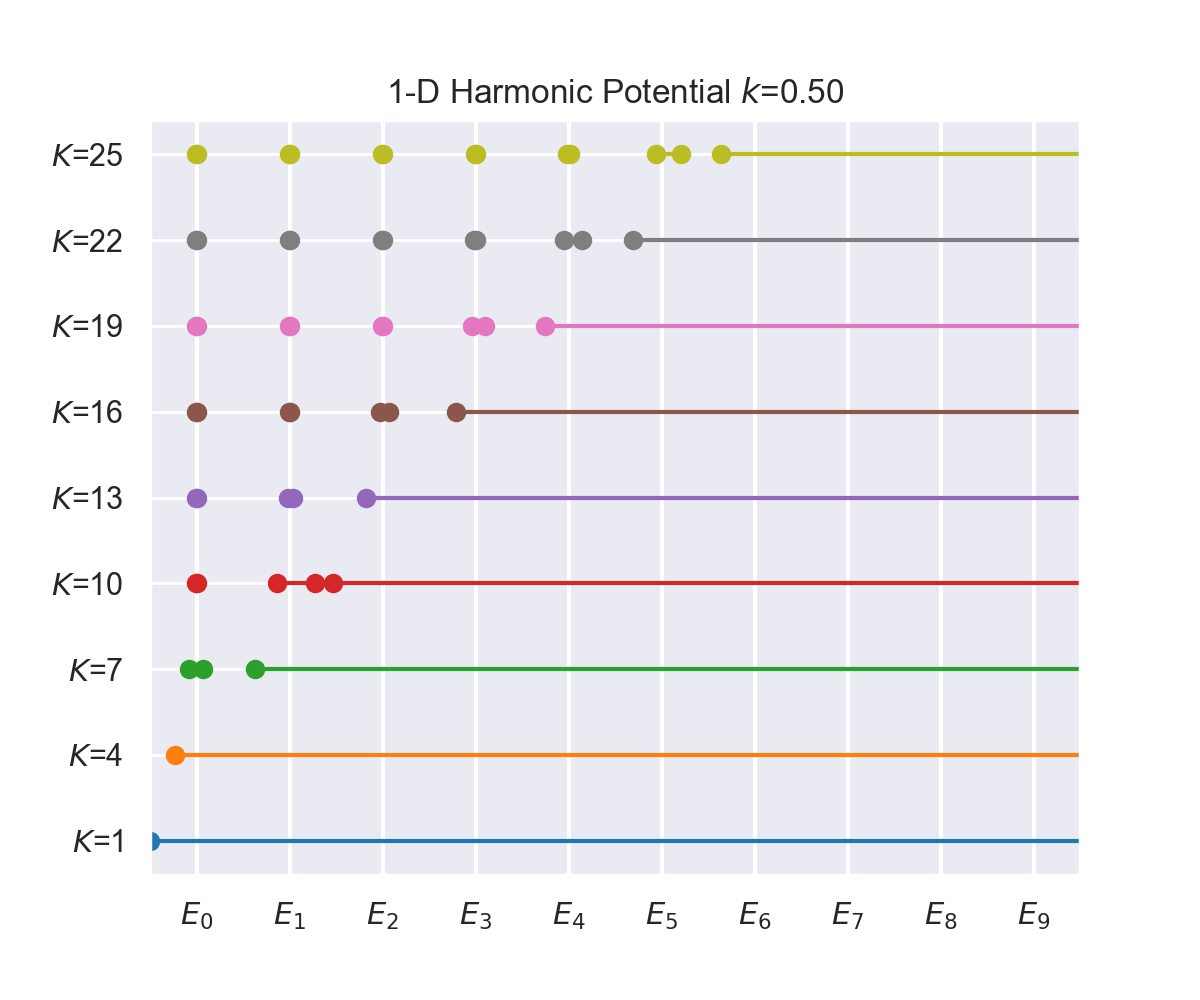
\includegraphics[scale=0.47]{result_N25_k0.50.png}\label{hp25a}
}\qquad
\subfloat[$k=1.00$]{
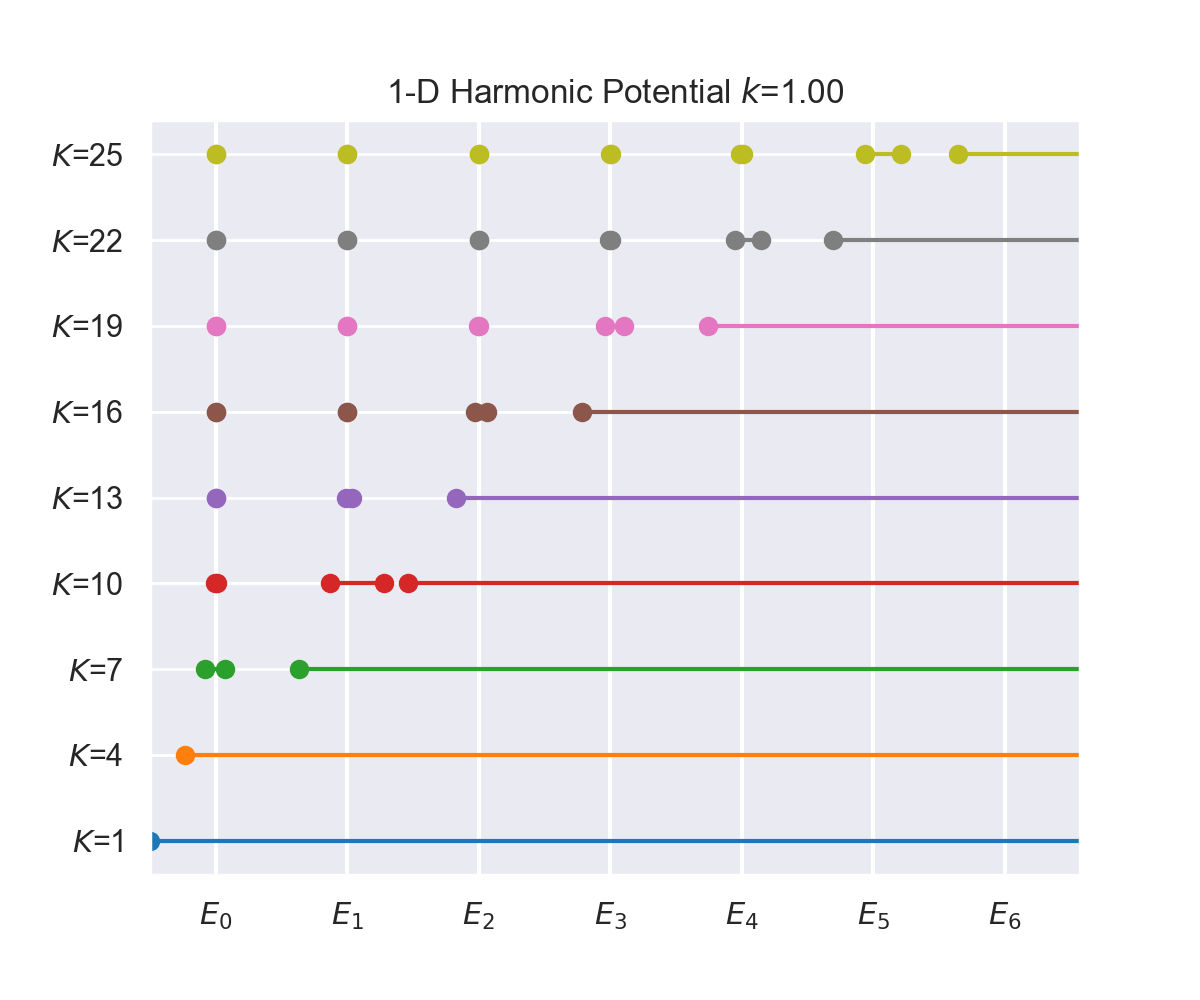
\includegraphics[scale=0.47]{result_N25_k1.00.png}\label{hp25b}
}
\caption{Harmonic potential for different $k$ with maximum Hankel matrix size $25\times 25$. The plot range of x-axis for two plots are the same, the labels on y-axis are the maximum size of Hankel matrix computed. The white vertical lines indicate the analytic energy eigenvalues. The x-labels are the corresponding analytic energy eigenvalues.}
\end{figure}
\begin{figure}[!htb]
\centering
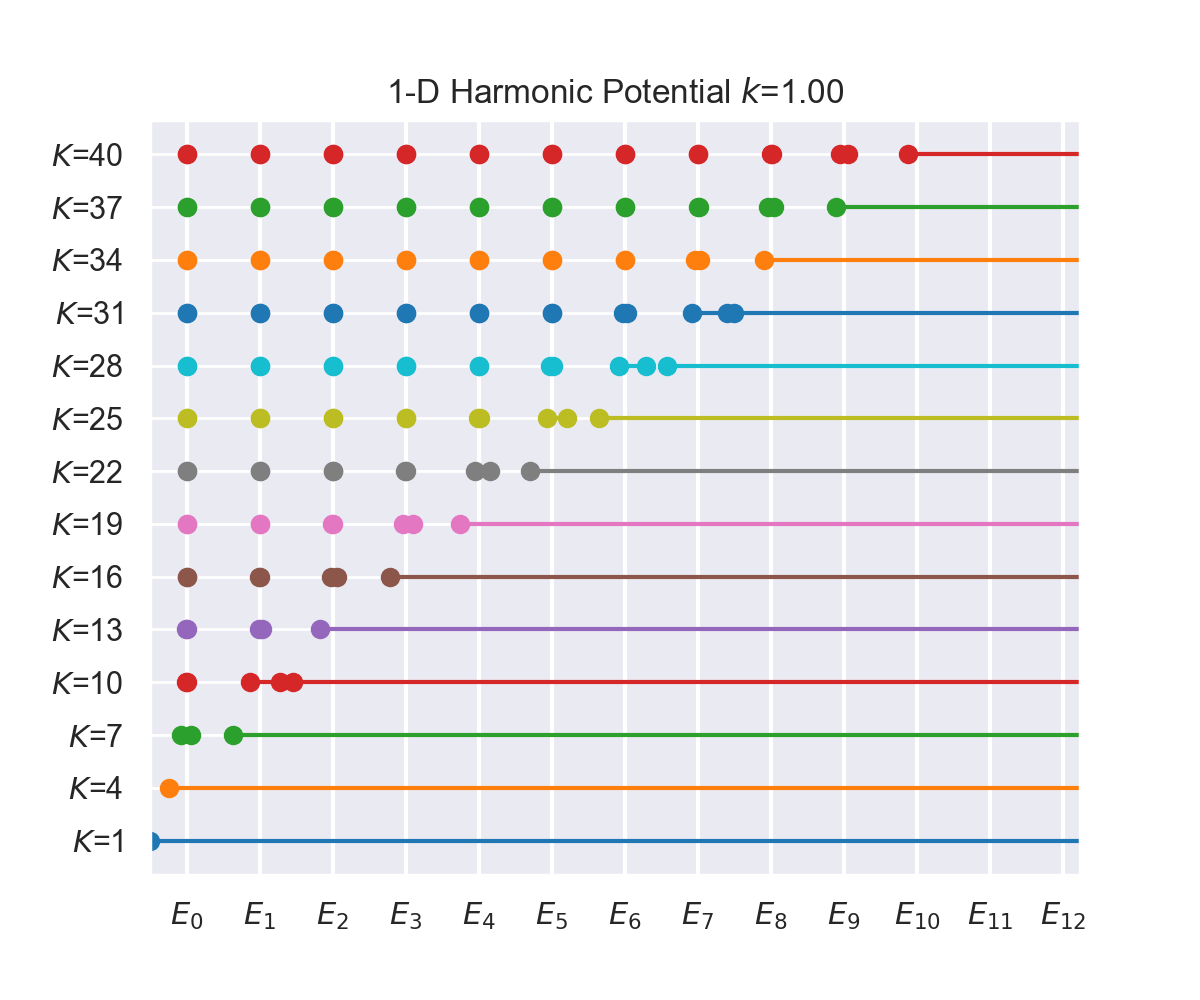
\includegraphics[scale=0.8]{result_N40_k1.00.png}
\caption{Harmonic potential for different $k=1.00$ with maximum Hankel matrix size $40\times 40$. Due to the limitation of hardware computing power, when computing only the size $K=40$ already requires about 4 hours.}
\label{hp40}
\end{figure}



Fig.\ref{hp25a} and fig.\ref{hp25b} show the allowed energy eigenvalues intervals such that the determinants of all submatrices of Hankel matrix are semi-positive. The allowed intervals indeed shrink to the analytic energy eigenvalues $E_n$. From fig.\ref{hp40}, we see that as about $3$ more size larger of Hankel matrix considered, another new excited energy eigenvalue appears.

% -------------------------------------------------------------------
\section{Coulomb Potential (Hydrogen-like Atom)}\label{sec:3}

The Coulomb potential of Hydrogen-like Atom is
\begin{equation}
    V(r)=\frac{q_1q_2}{4\pi\epsilon_0 r}=-\frac{k}{r}
\end{equation}
Take Hydrogen Atom for example, $q_1=q_{\text{proton}}=e$ and $q_2=q_{\text{electron}}=-e$ $\Rightarrow$ $k=\frac{e^2}{4\pi\epsilon_0}$. If we consider a Hydrogen-like Atom with angular momentum quantum number $l$, and set $m=\hbar=1$, the Hamiltonian becomes
\begin{equation}
    H(r)=\frac{1}{2}P^2_r+\frac{l(l+1)}{2r^2}-\frac{k}{r}
\end{equation}
We can view the non-momentum part as effective potential, i.e.,
\begin{align}
V_{\text{eff}}(r)&=\frac{l(l+1)}{2r^2}-\frac{k}{r}\\
V^\prime_{\text{eff}}(r)&=-\frac{l(l+1)}{r^3}+\frac{k}{r^2}
\end{align}
Since $P_r$ is the canonical momentum of $r$, it satisfies the commutator  relation $[r,P_r]=i$. We can transformed the Hydrogen-like Hamiltonian into an 1-dimensional problem with
\begin{align*}
    r &\rightarrow X\\
    P_r &\rightarrow P\\
    V_{\text{eff}}(r) &\rightarrow V(X)
\end{align*}
Substitute the Coulomb potential into eq.(\ref{recursion}), we get the recursion relation
\begin{equation}\label{h1}
    -E\langle r^s\rangle = 
    \frac{k(2s+1)}{2(s+1)}\langle r^{s-1}\rangle
    +[\frac{s(s-1)}{8}-\frac{sl(l+1)}{2(s+1)}]\langle r^{s-2}\rangle
\end{equation}
Similarly, $\langle r^0\rangle=1$. Take $s=0\Rightarrow \langle r^{-1}\rangle=-\frac{2E}{k}$. With $\langle r^{-1}\rangle$ and take $s=1\Rightarrow \langle r^1\rangle=-\frac{3k}{4E}-\frac{l(l+1)}{2k}$. We now transform the energy eigenvalues $E\rightarrow-\frac{1}{E}$, eq.(\ref{h1}) becomes
\begin{equation}
    \langle r^s\rangle = 
    \frac{k(2s+1)}{2(s+1)}E\langle r^{s-1}\rangle
    +[\frac{s(s-1)}{8}-\frac{sl(l+1)}{2(s+1)}]E\langle r^{s-2}\rangle
\end{equation}
We list the first few elements in Hankel matrix $M$ below (with transformation $E\rightarrow -\frac{1}{E}$)
\begin{align*}
    \langle r^0\rangle &= 1\\
    \langle r^1\rangle &= \frac{3Ek}{4}-\frac{l\left(l+1\right)}{2k}\\
    \langle r^2\rangle &= \frac{E \left(5 E k^{2} - 6 l \left(l + 1\right) + 2\right)}{8}\\
    \langle r^3\rangle &= \frac{E \left(35 E^{2} k^{4} - 60 E k^{2} l^{2} - 60 E k^{2} l + 50 E k^{2} + 12 l^{4} + 24 l^{3} - 12 l^{2} - 24 l\right)}{64 k}\\
    \langle r^4\rangle &= \frac{E^{2} \left(63 E^{2} k^{4} - 140 E k^{2} l^{2} - 140 E k^{2} l + 210 E k^{2} + 60 l^{4} + 120 l^{3} - 140 l^{2} - 200 l + 48\right)}{128}\\
\end{align*}
\begin{figure}[!htb]
\centering
\subfloat[$k=1.00$ and $l=1$]{
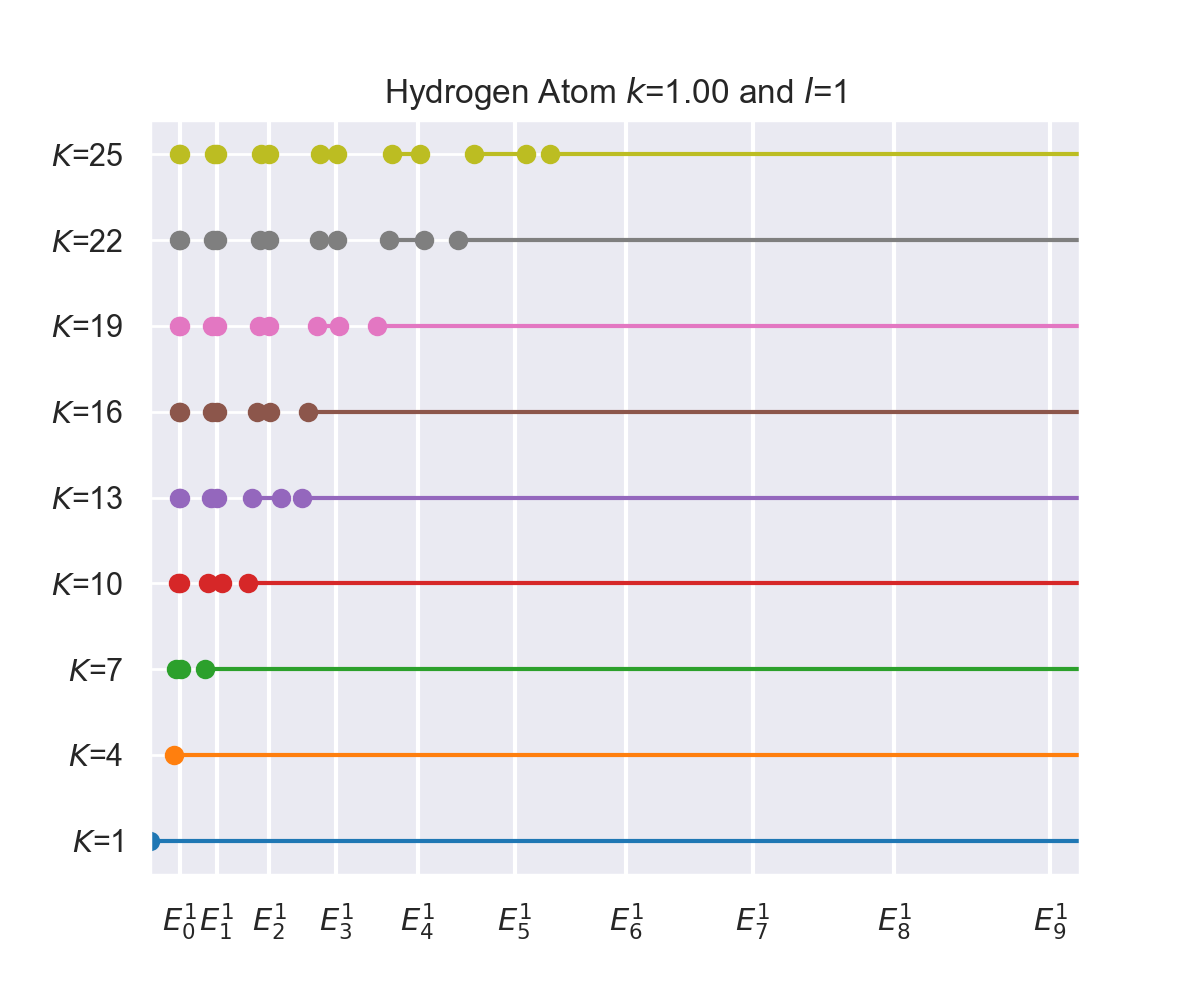
\includegraphics[scale=0.43]{result_N25_k1.00_l1.png}\label{cp25a}
}\qquad
\subfloat[$k=1.00$ and $l=2$]{
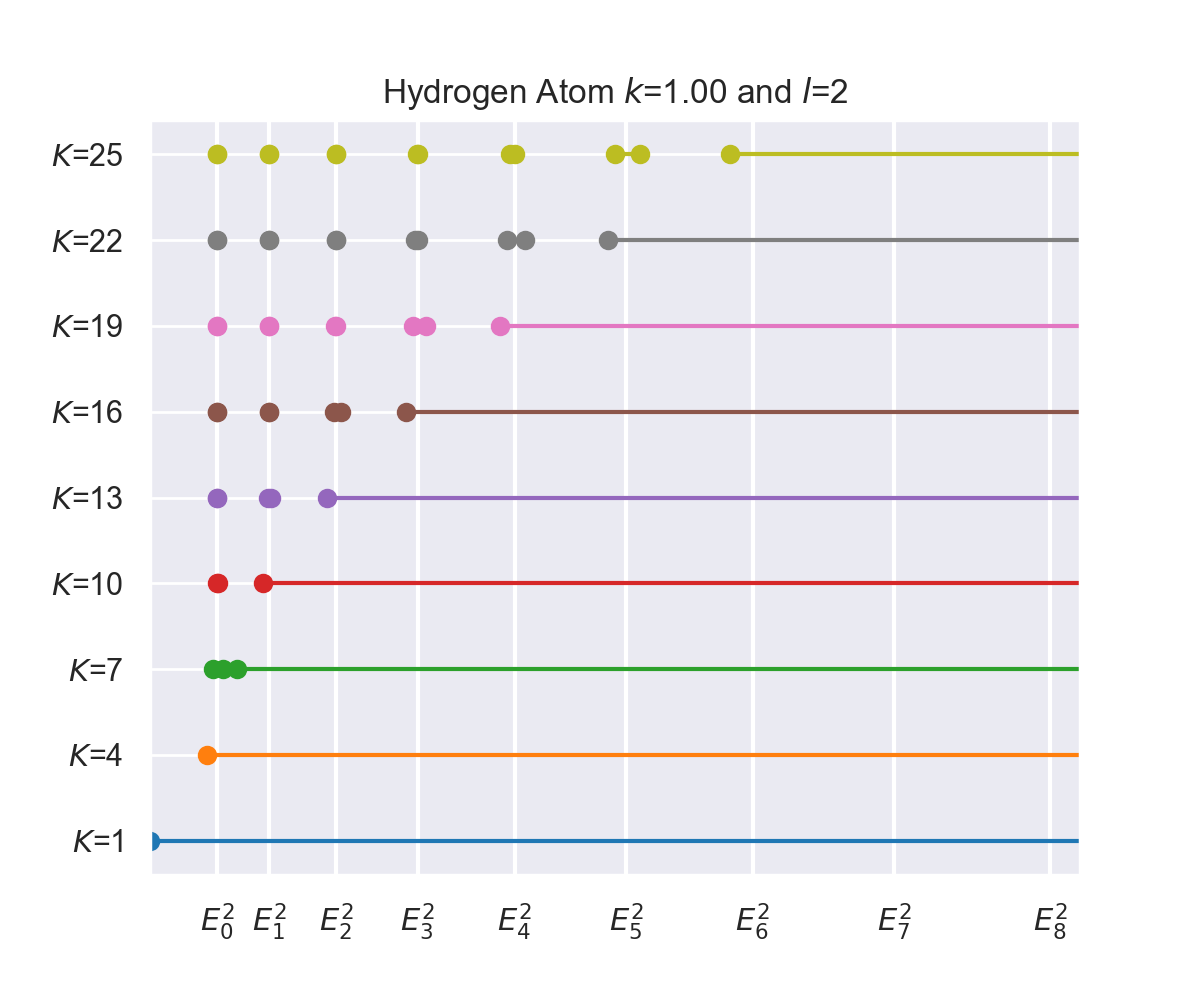
\includegraphics[scale=0.43]{result_N25_k1.00_l2.png}\label{cp25b}
}
\\
\subfloat[$k=1.00$ and $l=3$]{
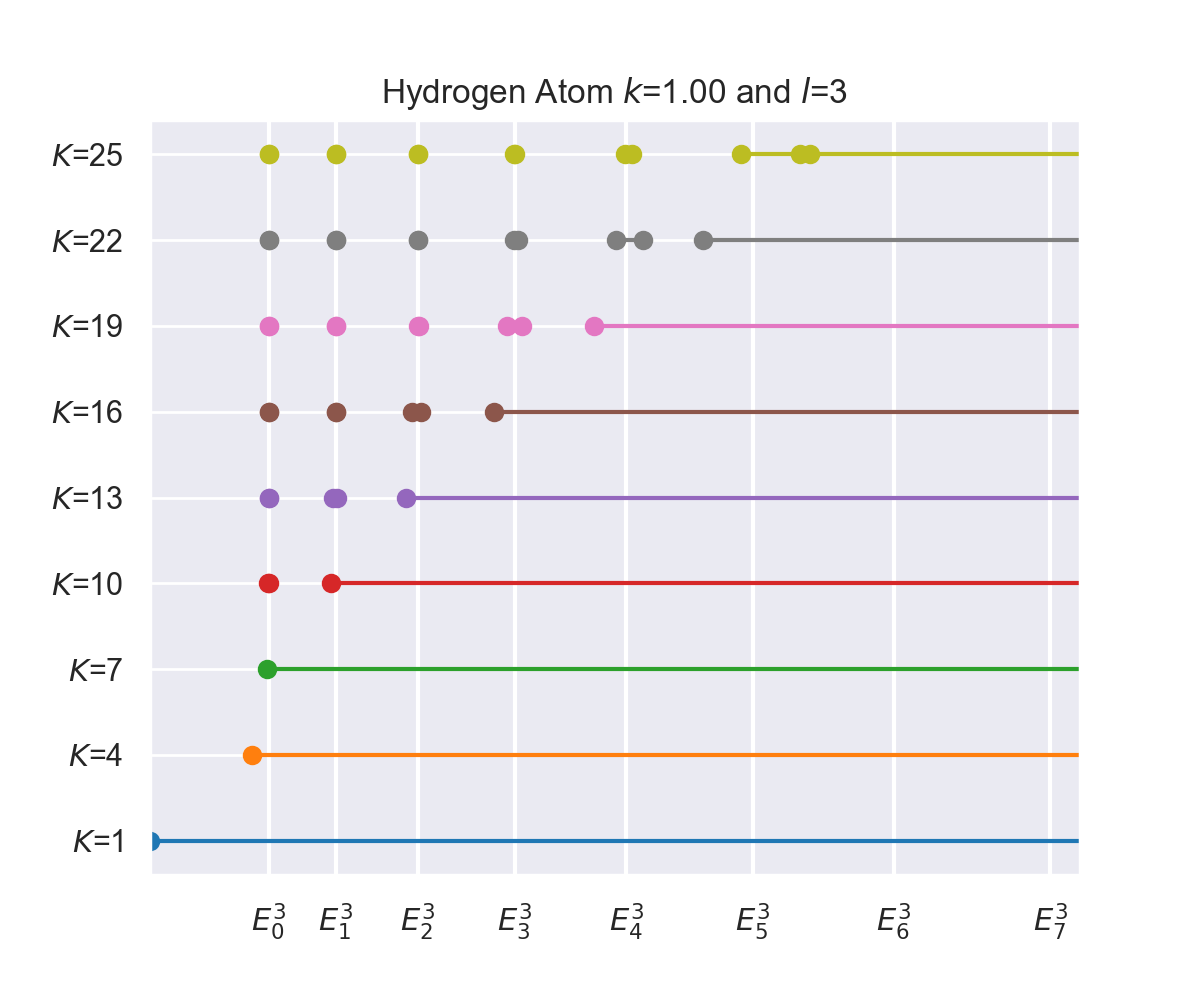
\includegraphics[scale=0.43]{result_N25_k1.00_l3.png}\label{cp25c}
}\qquad
\subfloat[$k=1.00$ and $l=4$]{
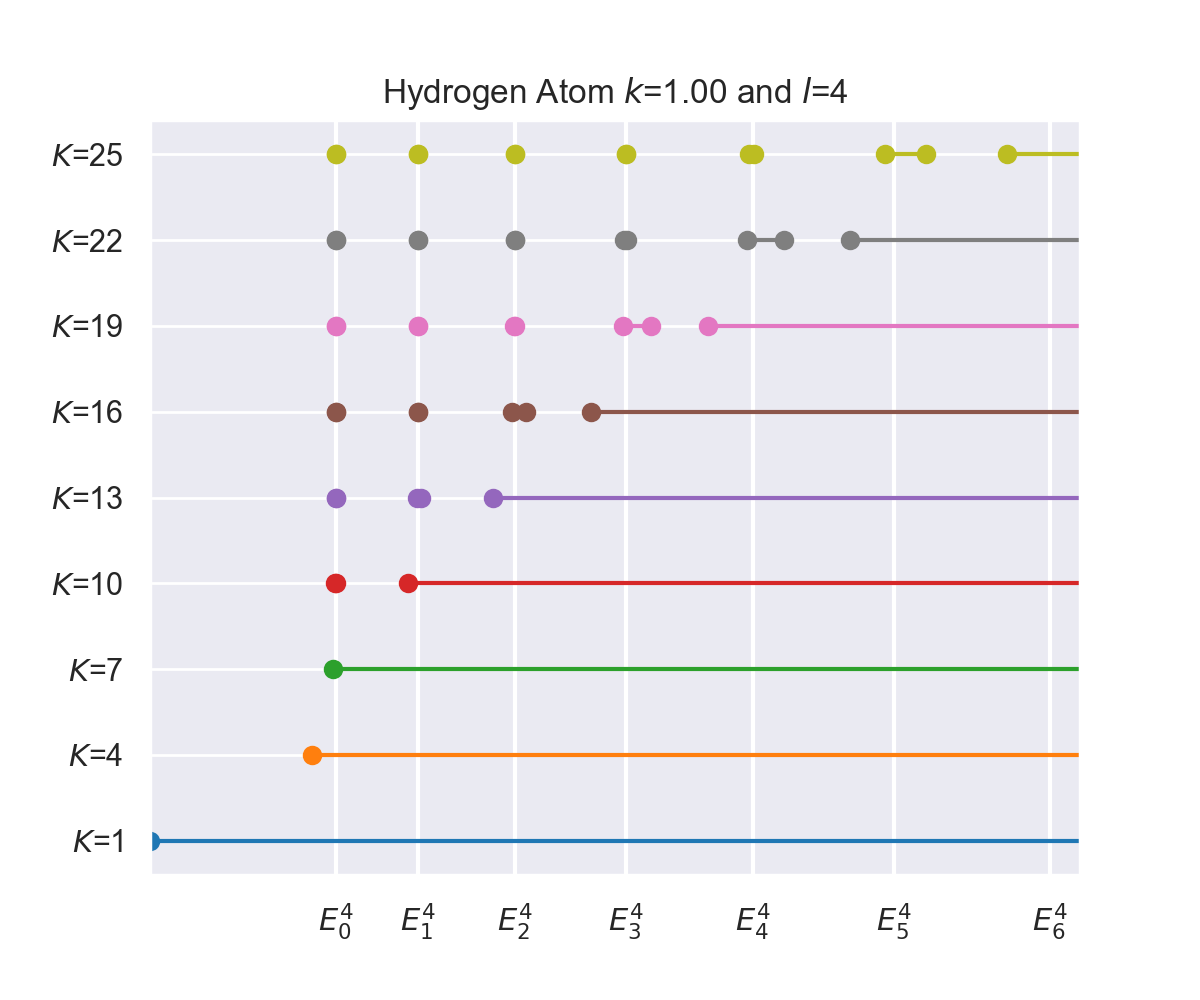
\includegraphics[scale=0.43]{result_N25_k1.00_l4.png}\label{cp25d}
}
\caption{Coulomb potential for different angular momentum quantum number $l$ with maximum Hankel matrix size $25\times 25$. The plot range of x-axis for four plots are the same, the labels on y-axis are the maximum size of Hankel matrix computed. The white vertical lines indicate the analytic energy eigenvalues. The x-labels are the corresponding analytic energy eigenvalues, with the superscript and the subscript indicate $l$ and $n_r$ respectively.}
\label{cp25}
\end{figure}

Fig.\ref{cp25} plots with different angular momentum quantum number $l$. Recall that we have transformed $E\rightarrow -\frac{1}{E}$, the original analytic energy becomes
\begin{equation}
    E^l_{n_r}(k)=-\frac{k^2}{2(n_r+l+1)^2} \longrightarrow E^l_{n_r}(k)=\frac{2(n_r+l+1)^2}{k^2}
    \qquad \text{with} \qquad n_r=0,1,2,3,...
\end{equation}
Note that $n_r$ is the radial quantum number, which indicates the index of allowed energy eigenvalues with a specific angular momentum quantum number $l$. The principal quantum number $n=n_r+l+1$ should be greater than the angular momentum quantum number $l$, i.e., $n>l$. That's why as $l$ getting larger, the lower allowed energy eigenvalues intervals are disappeared.

\textbf{Issue with $l=0$:} According to \cite{berenstein2021bootstrapping}, we both fail to use the Bootstrapping Method on $l=0$ case.

% -------------------------------------------------------------------
\section{First order approximated Yukawa Potential}\label{sec:4}

The original Yukawa potential in a simplified form is
\begin{equation}
    V(r)=-\frac{k}{r}e^{-ar}
\end{equation}
where we've set $m=\hbar=1$, and $a$ is some other positive scaling constant. Note that for $a=0$ case, it is just the trivial Coulomb potential. Substitute the Yukawa potential into eq.(\ref{recursion}), we get the recursion relation
\begin{equation}\label{y1}
    \frac{s(s+1)(s-1)}{4}\langle r^{s-2}\rangle + 2E(s+1)\langle r^s\rangle + k(2s+1)\langle r^{s-1}e^{-ar}\rangle - ak\langle r^s e^{-ar}\rangle=0
\end{equation}
Take the Taylor expansion of $e^{-ar}$, i.e., $e^{-ar}=1-ar+O(a^2)$, and keep $a$ to the first order in eq.(\ref{y1}), we get the approximated recursion relation
\begin{equation}
    -(E-ak)\langle r^s\rangle = 
    \frac{k(2s+1)}{2(s+1)}\langle r^{s-1}\rangle
    +[\frac{s(s-1)}{8}-\frac{sl(l+1)}{2(s+1)}]\langle r^{s-2}\rangle
\end{equation}
Compare the the recursion relation eq.(\ref{h1}) for Coulomb potential, we see that they only differ from a energy shift $E\rightarrow E-ak$. We can solved the approximated Yukawa potential with the same algorithm of Coulomb potential! The analytic energy eigenvalues become (before transformation)
\begin{equation}\label{ykapprox}
    E^l_{n_r}(a,k)=-\frac{k^2}{2(n_r+l+1)^2}+ak
\end{equation}
According to \cite{approxyukawa}, the approximated energy eigenvalues is given by
\begin{equation}\label{ykanaly}
    E^l_{n_r}(a,k)=-\frac{[k-a(n_r+l+1)^2]^2}{2(n_r+l+1)^2}
\end{equation}
When taking approximation to the first order of $a$, eq.(\ref{ykanaly}) indeed reduces to eq.(\ref{ykapprox}). By the same trick, let $E\rightarrow -\frac{1}{E-ak}$, then the elements of the Hankel matrix is exactly the same as Coulomb potential. Since the result is similar to Coulomb potential, we consider not to put the plotting result here.

% -------------------------------------------------------------------
\section{Discussion and Conclusion}\label{sec:5}
Bootstrapping Method provides us a new way to solve the energy eigenvalues, based on the consistency relation of Quantum Mechanics. Some issues still need to be studied, e.g., $l=0$ case in Coulomb potential, or some special potential like Yukawa potential.


% \newpage

\bibliographystyle{plain} % We choose the "plain" reference style
\bibliography{ref} % Entries are in the refs.bib file

\end{document}